\documentclass[12pt,oneside]{fithesis2}
\usepackage[english]{babel}       % Multilingual support
\usepackage[utf8]{inputenc}       % UTF-8 encoding
\usepackage[T1]{fontenc}          % T1 font encoding
\usepackage[                      % A sans serif font that blends well with Palatino
  scaled=0.86
]{berasans}
\usepackage[                      % A tt font if you do not like LM's tt
  scaled=1.03
]{inconsolata}
\usepackage[                      % Clickable links
  plainpages = false,               % We have multiple page numberings
  pdfpagelabels                     % Generate pdf page labels
]{hyperref}
\usepackage{blindtext}            % Lorem ipsum generator
\usepackage{amsmath}
\usepackage{mathtools}
\usepackage{scalefnt}
\usepackage{graphicx}
\usepackage{wrapfig}

 % Algorithms
\usepackage{algorithm}
%\usepackage[noend]{algpseudocode}
\usepackage{algpseudocode}

\thesislang{en}                   % The language of the thesis
\thesistitle{Scalable Parameter Synthesis from CTL Hypotheses}       % The title of the thesis
\thesissubtitle{Bachelor Thesis}  % The type of the thesis
\thesisstudent{Samuel Pastva}          % Your name
\thesiswoman{false}                % Your gender
\thesisfaculty{fi}                % Your faculty
\thesisyear{Spring \the\year}     % The academic term of your thesis defense
\thesisadvisor{prof. RNDr. Luboš Brim, CSc.}   % Your advisor


% Macros for definitions
% Assumptions
\newcommand{\as}[1][]{\ensuremath{\mathcal{A}_{#1}}}
\newcommand{\asemt}{\as[\perp]}
\newcommand{\ain}{\mathcal{A}_{in}}
\newcommand{\ASphi}{\ensuremath{AS_{\kf{i}{}}^\varphi}}
\newcommand{\sem}{\ensuremath{\mathcal{C}_{\kf{i}{}}^\varphi}}

% Algorithm
\newcommand{\method}[1]{\textnormal{\textsc{#1}}}

%True, false
\newcommand{\true}{\ensuremath{\texttt{tt}}}
\newcommand{\false}{\ensuremath{\texttt{ff}}}

% Kripke
\newcommand{\ks}[1][]{\ensuremath{\mathcal{K}_{#1}}}
\newcommand{\kf}[2]{\ensuremath{\mathcal{F}^{#2}_{#1}}}
\newcommand{\fullKs}{\ensuremath{ \ks = (\params, S, S_0, \trans{}, L) }}
\newcommand{\fullKf}[2]{\ensuremath{ \kf{#1}{#2} = (\params, S_{#1}, I_{i}, \trans{}_{#1}, L_{#1}) }}
\newcommand{\trans}[1]{\stackrel{#1}{\rightarrow}}
\newcommand{\params}{\mathcal{P}}

%Temporal
\newcommand{\eu}[2]{\ensuremath{\mbox{E} #1 \mbox{U} #2 }}
\newcommand{\au}[2]{\ensuremath{\mbox{A} #1 \mbox{U} #2 }}
\newcommand{\ex}[1]{\ensuremath{\mbox{EX} #1}}
\newcommand{\ax}[1]{\ensuremath{\mbox{AX} #1}}
\newcommand{\ef}[1]{\ensuremath{\mbox{EF} #1}}
\newcommand{\af}[1]{\ensuremath{\mbox{AF} #1}}
\newcommand{\eg}[1]{\ensuremath{\mbox{EG} #1}}
\newcommand{\ag}[1]{\ensuremath{\mbox{AG} #1}}

 \algblockdefx{ForAllPar}{EndForPar}[2]%
 {\textbf{for all }#1 \textbf{do in parallel} #2}%



\begin{document}
  \FrontMatter                    % The front matter
    \ThesisTitlePage                % The title page
    \begin{ThesisDeclaration}       % The declaration
      \DeclarationText
      \AdvisorName
    \end{ThesisDeclaration}
    \begin{ThesisThanks}            % The acknowledgements (optional)
      I would like to thank all members of Systems Biology Laboratory for their support, patience and for giving me insight into systems biology. Namely, I would like to thank my advisor, prof. RNDr. Luboš Brim, CSc., for inviting me to the laboratory and advising me on this thesis, RNDr. David Šafránek, Ph.D. for advising me about various biochemical models and  Mgr. Martin Demko for his information about existing Biodivine code base.
      
      I would also like to thank my family and friends, who supported me throughout my bachelor's studies.
    \end{ThesisThanks}
    \begin{ThesisAbstract}          % The abstract
      The main goal of this thesis is to design and implement a parallel and distributed memory algorithm for computing the parameter synthesis problem for biochemical systems and CTL hypotheses. The resulting algorithm is based on coloured CTL model checking. The applicability and scalability of the algorithm is successfully demonstrated on biochemical models based on ordinary differential equations. We also discuss possible heuristics for state space partitioning of these models.
    \end{ThesisAbstract}
    \begin{ThesisKeyWords}          % The keywords
		Coloured Model Checking, CTL, Distributed Memory, Parameter Synthesis Problem, Systems Biology, ODE Model, Thomas Network
    \end{ThesisKeyWords}
    \tableofcontents                % The table of contents
%   \listoftables                   % The list of tables (optional)
%   \listoffigures                  % The list of figures (optional)
  
  \MainMatter                     % The main matter
    \chapter{Introduction}          % Chapters
	
		With advancements in human knowledge about biochemical processes in living organisms, the complexity of experiments and theories needed to advance this knowledge even further is constantly increasing. This makes the search for computational models describing dynamics of biochemical processes a key step towards understanding of the behavioural and physiological phenotypes occurring in biology.
		
		Complex biochemical processes occurring in living organisms are usually dependent on high number of parameters, such as reaction rates or concentration values. While the qualitative aspects of some of these processes are already known, the quantitative aspects are usually hard to measure and therefore cannot be easily determined. This leaves values of many parameters in biochemical systems uncertain or completely unknown.
		
		The aim of the \emph{parameter synthesis} is to find a set of values of these unknown parameters, such that these valuations meet a stated dynamical constraints. These dynamical constraints can be captured in terms of temporal logic formulas. 
				
		The problem whether model meets specified temporal specification is well explored in computer science and can be solved using \emph{model checking} \cite{clarke}. Several methods for parameter synthesis based on model checking have already been proposed with various modelling techniques and temporal logic in mind \cite{ieee,batt,gilbert,donze,jha}.
		
		In this work, in order to express biologically relevant hypothesis, we focus on the branching time based logic, CTL. This is because many biological properties, such as multi-stability, need branching time operators to express them properly. It is very difficult or even impossible to express these properties correctly in linear time based logic, such as LTL. 
		
		Another advantage of CTL logic is that the particular procedure of model checking does not rely on initial conditions, effectively identifying all states where given property is satisfied. This leads to a global analysis of the model, as opposed to LTL model checking procedure, which requires a single initial state.
				
		This work proposes a new method of solving the parameter synthesis problem based on the CTL model checking. To tackle the problem of state space and parameter state explosion, we base our algorithm on distributed CTL model checking as defined in \cite{assumptions} and coloured model checking as introduced in \cite{ieee}. We also provide an implementation on which we demonstrate the applicability and scalability of this new algorithm. 		
		
		The work is divided into seven chapters. Second and third chapter introduce the notion of Parametrised Kripke Structures, Kripke Fragments, State Space Partitioning and provide a short overview of employed modelling techniques. Fourth chapter describes the distributed algorithm itself. Fifth chapter discusses the details of the implementation. Finally, sixth chapter is dedicated to scalability and case study discussion.
				
	\chapter{Parameter synthesis problem}
	
		In this chapter, we define formalisms which enable us to describe parametrised models and temporal constrains on these models. We use these formalisms the define the parameter synthesis problem. We also discuss relationship between CTL logic and approximated models.
		
		\section{Parametrised Kripke Structure}
	
			As an input of our algorithm, we expect a parametrised Kripke Structure as defined in \cite{ieee}. Parametrised Kripke Structure is a tuple $\fullKs$ where
			
			\begin{itemize}
				\item $\params$ is a finite set of parameters (all possible parameter valuations)
				\item $S$ is a finite set of states
				\item $S_0 \subseteq S$ is a set of initial states
				\item $\trans{} \subseteq S \times \params \times S$ is a transition relation labelled by parameter valuations 
				\item $L: S \rightarrow 2^{AP} $ is a labelling function from states to sets of atomic propositions which are true in such states
			\end{itemize} 		
			
			We write $ s \trans{p} s' $ when $ (s, p, s') \in \trans{} $. We also write $ s \trans{} s'$ when $\exists p \in \params : (s, p, s') \in \trans{} $. Note that fixing a valuation $p \in \params$ reduces the Parametrised Kripke Structure $\ks$ to concrete, non-parametrised Kripke Structure $\ks(p) = (S, S_0, \trans{p}, L)$.
						
		\section{CTL Logic}
		
			\label{sec:ctl}
			For various biochemical models, the idea of branching time is suitable to express interesting properties of these models. Examples of such properties are given in section \ref{sec:case}. Therefore, we use the Computation Tree Logic (CTL) \cite{clarke} as means of hypotheses formulation. 

			CTL syntax is defined inductively upon set of atomic propositions $AP$:
			
			\begin{equation}
				\varphi ::= 
					true \mid
					false \mid
					Q \mid 
					\neg \varphi_1 \mid 
					\varphi_1 \wedge \varphi_2 \mid
					\ex{\varphi_1} \mid
					\eu{\varphi_1}{\varphi_2} \mid
					\au{\varphi_1}{\varphi_2}			
			\end{equation}
	
			Here $Q$ is an atomic proposition from set $AP$.			
			
			Sometimes, we will use parentheses to make complex formulas easily readable, but they will in no way be used to modify the meaning of formula or priority of operators.
			
			We also allow following standard abbreviations to make formulas more easily readable. Note that these abbreviations are not implemented directly in the algorithm. They are replaced with their equivalent representation prior computation.
			
			\begin{itemize}
				\item $ \ax{\varphi} = \neg \ex{ \neg \varphi } $
				\item $ \ef{\varphi} = \eu{(true)}{\varphi} $
				\item $ \eg{\varphi} = \neg \au{(true)}{\neg \varphi} $
				\item $ \af{\varphi} = \au{(true)}{\varphi} $
				\item $ \ag{\varphi} = \neg \eu{(true)}{\neg \varphi}$
			\end{itemize}
			
			Abbreviations to allow other boolean operators like implication or equivalence can also be used. 			
			
			Let $\varphi$ be a CTL formula. We write $cl(\varphi)$ to denote the set of all sub-formulas of $\varphi$ and $tcl(\varphi)$ to denote the set of all temporal sub-formulas of $\varphi$. By $|\varphi|$ we denote the size of formula $\varphi$.
			
			We assume CTL semantics over non-parametrised Kripke structures as defined in \cite{clarke}.

		\section{Parameter Synthesis Problem}
			
			Parameter synthesis problem is defined in following way. Suppose we are given a parametrised Kripke structure $\fullKs$ and a CTL formula $\varphi$. For each state $s \in S$ let $ P_s = \{ p \in \params \mid s \models_{\ks(p)} \varphi \} $, where $s \models_{\ks(p)} \varphi$ denotes, that $\varphi$ is satisfied in the state $s$ of $\ks(p)$. The parameter synthesis problem requires to compute the function $\mathcal{M}_{\varphi}^{\ks} : S \rightarrow 2^\params $ such that $\mathcal{M}_{\varphi}^{\ks}(s) = P_s$. Often we are especially interested in computing the set of all parameters for which the property holds in some of the initial states: $\cap_{s\in S_0}\mathcal{M}_\varphi^{\mathcal K}(s)$. We can sometimes omit the $\varphi$ and $\ks$ when they are clear from the context.	
				
		\section{CTL Logic and Model Approximation}
		
			In model checking, some modelling approaches suffer from over or under approximation. We say that model is over-approximated if all feasible paths are contained in the model, but it can also contain paths that are not feasible in the situation the model is describing. Symmetrically, we say that model is under-approximated when all paths in the model are feasible in the modelled situation, but not all feasible paths have to be contained in the model. 
			
			It is important to discuss this relationship between CTL and approximated models, because it is much more complicated compared to linear-time logic, since CTL allows for universal and existential quantification mixing.
			
			We say that CTL formula is \emph{universal} or that it belongs to ACTL when it only contains universal temporal operators and no negation. Symmetrically, we say that CTL formula is \emph{existential} or that it belongs to ECTL when it only contains existential temporal operators and no negation.
			
			Observe that the truth of ACTL properties is preserved in over-approximated models. In other words, if an ACTL property holds in an over-approximated model, it must also hold in a model without approximation. However, their falsity cannot be guaranteed, because the false paths may falsify the property in states where it would be normally true. Similarly, the falsity of ECTL properties in over-approximated models is preserved, but the truth is not. In this case, the existence of false paths can introduce states where ECTL property holds solely due to these false paths.
			
			Symmetrically, for under-approximated models, we observe that the falsity of ACTL and the truth of ECTL is preserved. But due to similar arguments, we can't say anything about their counterparts.
			
			If we allow full CTL, in general, we can't make any assumptions about results obtained from either under- or over-approximated systems. This is caused by mixing of existential and universal quantification which leads to results that may be spurious and incomplete at the same time. Therefore, no conclusions can be made without further investigation and validation of such results.
			
	\chapter{State Space Distribution}
		
		In this chapter, we describe the process of state space distribution using the notion of Kripke fragments and CTL assumption semantics. 
				
		\section{Kripke Fragments}
		
			Due to the state space explosion, given parametrised Kripke structure can be very large and therefore impossible to fit into memory of one computer. In order to solve parameter synthesis problem for such structures, we have to distribute the state space across several computational nodes. To this end, we adapt the notion of par\-am\-etrised Kripke fragments as described in \cite{assumptions}.
			
			A parametrised Kripke structure $\ks$ can be divided into several parametrised Kripke fragments $\kf{1}{\ks}, \kf{2}{\ks}, \cdots , \kf{N}{\ks}$ using a partition function $f : S \rightarrow \{1, \cdots , N \}$. Parametrised Kripke fragment with identifier $i$ over Kripke structure $\fullKs$ is then defined as a tuple $\fullKf{i}{\ks}$ where:
			
			\begin{itemize}
				\item $\params$ is a finite set of all parameters
				\item $S_{i} = \{ s \in S \mid f(s) = i \vee \exists s'\in S : (s' \trans{} s \wedge f(s') = i \}$ is a subset of original state space which belongs to this fragment
				\item $I_{i} = S_i \cap S $ is a set of all initial states that belong to the fragment
				\item $\trans{}_{i} = \{ (s, p, s') \in \trans{} \mid s \in S_{i} \wedge s' \in S_{i} \wedge (f(s) = i \vee f(s') = i) \}$ is a subset of original transition relation reduced to only relevant states (not required to be total)
				\item $L_{i} = \{ (s, l) \in L \mid f(s) = i \}$ is a subset of original labelling function relevant to this fragment
			\end{itemize}
						
			In the following text, we will often omit the superscript $\ks$ if it is clear from context.
						
			Intuitively, Kripke fragment represents a subset of the original Kripke structure. It contains all states specified by the partition function with all their direct successors and all corresponding transitions. A state in fragment has either none or exactly the same successors as in $\ks$.
			
			We write $border(\kf{i}{\ks}) =  \{ s\in S_i \mid \neg \exists (p,s').s\trans{p}s'\}$ to denote the set of border states. Intuitively, these states represent the remaining portion of the state space which is stored in memory of other processes and is not directly accessible. We say that state is an \emph{internal state} if it is not a border state. For each border state, there is a copy of this state that is internal in another fragment. We also define a set of cross edges as $cross(\kf{i}{\ks}) = \{ (s, p, s') \in \trans{}_{i} \mid s' \in border(\kf{i}{\ks}) \}$. Intuitively, these are edges leading from internal states to border states. 
			
			\begin{figure}
			  \begin{center}
				 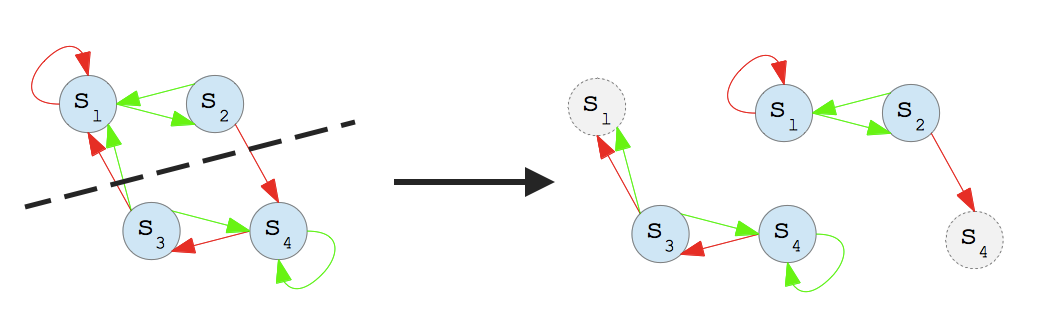
\includegraphics[scale=.3]{partition.png}
				\label{fig:genmodel}
				\caption{Example of the state space partitioning. Gray states are border states. }
				\end{center}
			\end{figure}


			Note that for a constant partition function $f(s) = 1$ and any given Kripke structure, the partitioning results in one fragment with an unchanged state space and an unchanged transition relation (The sets of border states and cross edges are empty for the resulting fragment). Similarly, for every Kripke structure, there exists a partition function for which $N = |S|$ and every resulting fragment contains only one internal state. Under such partitioning, all edges are cross edges. 
			
			In the worst case (connected graphs), such partitioning results in fragments with $|S| - 1$ border states and one internal state. Therefore we can assume that $\sum\limits_{i=1}^N | S_i | \leq |S|^2 $, hence the number of introduced border states is at worst quadratic in terms of original state space. The number of internal states remains always the same.

			This increase seems rather high, however, it is important to note that this also requires one process for each internal state. In real life scenarios, the number of states per process is usually much higher. Also note that the representation of border state in memory is usually much simpler (and smaller) than representation of internal state, so even a distribution with high border state count can be beneficial in terms of memory consumption. 								
			
			The number of border states and cross edges is also highly dependent on the partition function. It is usually best to design the partition function with specific model or modelling approach in mind in order to achieve optimal workload distribution. We will discuss different partition functions later in chapter \ref{chap:partitioning}. 
			
			For each Kripke fragment $\kf{i}{}$, we define a function $successors \subseteq S_{i} \rightarrow S_{i} \times 2^\params$ to denote the set of all successor states and relevant colour sets that enable such transition.
			
			\begin{center}
				$successors(s) = \{(s', P) \in S_{i} \times 2^\params \mid s \trans{}_{i} s' \wedge P = \{p \in \params \mid (s, p, s') \in \trans{}_i \}\} $
			\end{center}
			
			Symmetrically, we define a function $predecessors \subseteq S_{i} \rightarrow S \times 2^\params$ to denote the set of all predecessor states and relevant colour sets that enable such transition.
			
			\begin{center}
				$predecessors(s) = \{(s', P) \in S \times 2^\params \mid s' \trans{} s \wedge P = \{p \in \params \mid (s', p, s) \in \trans{} \}\} $
			\end{center}						
			
			Note that the function $predecessors$ can actually return states that are not contained in the state space owned by the fragment. This function is used later in the algorithm to reduce the possible communication overhead, but is not crucial to the asymptotic complexity of the algorithm. This function can be easily computed prior to the actual model checking when information about whole state space is still available.
			
		\section{Assumption Semantics}
		
			Classic interpretation of CTL formulas is not adequate for Kripke fragments. In order to accommodate for possible non-totality and distributed nature of the Kripke fragments over Kripke structure $\ks$, we introduce the assumption function $\as : \params \times S \times cl(\varphi) \rightarrow Bool $. The values $\as(s, p, \varphi_1)$ are called assumptions. We use the notation $\as(p, s, \varphi_1) = \perp $ to say that the value of $\as(s, p, \varphi_1)$ is undefined. By $\asemt$ we denote assumption function which is undefined for all inputs.
			
			Intuitively, $\as(s, p, \varphi_1) = \true$ when we can assume that $\varphi_1$ holds in a state $s$ for parameter valuation $p$, $\as(s, p, \varphi_1) = \false$ when we can assume that $\varphi_1$ does not hold in state $s$ for parameter valuation $p$ and $\as(s, p, \varphi_1) = \perp$ when we cannot assume anything about validity of $\varphi_1$ in state $s$ for parameter valuation $p$. We write $\ASphi$ to denote the set of all assumption functions for a formula $\varphi$ and parametrised Kripke fragment $\kf{i}{}$.
			
			Undefined values are important in CTL semantics over dis\-trib\-uted fragments, since such values can be used in places where validity of formula cannot be computed because it depends on information stored in another fragment which has not been received yet. However, a correct model checking algorithm should always provide a definitive answer for all states and parameter valuations in finite time.
			
			We consider a new semantic function $\sem: \ASphi \rightarrow \ASphi$ that takes an input assumption function $\ain$ and returns a new assumption function  $\as$. If $ s \in \mathit{border}(\kf{i}{})$ then $\as(p,s,\varphi) = \ain(p,s,\varphi)$.  If $ s \notin \mathit{border}(\kf{i}{})$ then $\as(p,s,\varphi)$ is defined recursively:
		
\begingroup		
\scalefont{0.9}{
\begin{equation*}
	\as(p, s, Q) = 
   	\begin{dcases}
    	\begin{split}
			\true
      	\end{split}
      & \text{\parbox{8cm}{$Q \in L_i(s)$}} \\
      	\begin{split}
       		\false
      	\end{split}
      & \text{otherwise}
   	\end{dcases}
\end{equation*}		
}				
\endgroup
			
\begingroup			
\scalefont{0.9}{
\begin{equation*}
	\as(p, s, \neg \varphi_1) = 
   	\begin{dcases}
    	\begin{split}
			\true
      	\end{split}
      & \text{\parbox{8cm}{$\as(p, s, \varphi_1) = \false$}} \\
      	\begin{split}
       		\false
      	\end{split}
      & \text{\parbox{8cm}{$\as(p, s, \varphi_1) = \true$}} \\
      	\begin{split}
       		\perp
      	\end{split}
      & \text{otherwise}
   	\end{dcases}
\end{equation*}		
}	
\endgroup
								
\begingroup
\scalefont{0.9}{
\begin{equation*}
	\as(p, s, \varphi_1 \wedge \varphi_2) =
   	\begin{dcases}
    	\begin{split}
			\true
      	\end{split}
      & \text{\parbox{8cm}{$\as(p, s, \varphi_1) = \true $ and $ \as(p, s, \varphi_2) = \true$}} \\
      	\begin{split}
       		\false
      	\end{split}
      & \text{\parbox{8cm}{$\as(p, s \varphi_1) = \false $ or $ \as(p, s, \varphi_2) = \false$}} \\
      	\begin{split}
       		\perp
      	\end{split}
      & \text{otherwise}
   	\end{dcases}
\end{equation*}		
}	
\endgroup

\begingroup			
\scalefont{0.9}{
\begin{equation*}
	\as(p, s, \ex{\varphi_1}) =
   	\begin{dcases}
    	\begin{split}
			\true
      	\end{split}
      & \text{\parbox{8cm}{$\exists s' \in S_i : s \trans{p}_i s' \wedge \as(p, s', \varphi_1) = \true$}} \\
      	\begin{split}
       		\false
      	\end{split}
      & \text{\parbox{8cm}{$\forall s' \in S_i : s \trans{p}_i s' \Rightarrow \as(p, s', \varphi_1) = \false$}} \\
      	\begin{split}
       		\perp
      	\end{split}
      & \text{otherwise}
   	\end{dcases}
\end{equation*}		
}	
\endgroup

\begingroup			
\scalefont{0.9}{
\begin{equation*}
	\as(p, s, \eu{\varphi_1}{\varphi_2}) =
   	\begin{dcases}
    	\begin{split}
			\true
      	\end{split}
      & \text{\parbox{8cm}{exits a p-path $\pi = s_0s_1 s_2
                  \ldots$ with $s=s_0$ such that $\exists x < |\pi|$ such that 
                  (either $\as(p, s_x, \varphi_2) = \true$ or [$s_x \in border(\kf{i}{})$ and $\as(p, s_x,  \eu{\varphi_1}{\varphi_2}) = \true])$, and $\forall 0 \leq y < x : \as(p, s_y, \varphi_1) = \true$ }} \\
      	\begin{split}
       		\false
      	\end{split}
      & \text{\parbox{8cm}{for all p-paths $\pi = s_0s_1 s_2
                  \ldots$ with $s=s_0$ either $\exists x < |\pi|$ such that 
                  $(\as(p, s_x, \varphi_1) = \false$ and $\forall y \leq x : \as(p, s_y, \varphi_2) = \false)$ or $[ \forall x < |\pi| : \as(p, s_x, \varphi_2) = \false $ and $( |\pi| = \infty $ or $( s_{|\pi| - 1} \in border(\kf{i}{}) $ and $ \as(p, s_{|\pi| - 1}, \eu{\varphi_1}{\varphi_2}) = \false ))]$ }} \\
      	\begin{split}
       		\perp
      	\end{split}
      & \text{otherwise}
   	\end{dcases}
\end{equation*}		
}	
\endgroup

\begingroup			
\scalefont{0.9}{
\begin{equation*}
	\as(p, s, \au{\varphi_1}{\varphi_2}) =
   	\begin{dcases}
    	\begin{split}
			\true
      	\end{split}
      & \text{\parbox{8cm}{for all p-path $\pi = s_0s_1 s_2
                  \ldots$ with $s=s_0$ such that $\exists x < |\pi|$ such that 
                  $[$ either $\as(p, s_x, \varphi_2) = \true$ or $(s_x \in border(\kf{i}{})$ and $\as(p, s_x,  \au{\varphi_1}{\varphi_2}) = \true)]$, and $\forall 0 \leq y < x : \as(p, s_y, \varphi_1) = \true$ }} \\
      	\begin{split}
       		\false
      	\end{split}
      & \text{\parbox{8cm}{exists a p-path $\pi = s_0s_1 s_2
                  \ldots$ with $s=s_0$ and an index $x < |\pi|$ such that: 
                  $(\as(p, s_x, \varphi_1) = \false$ and $\forall y \leq x : \as(p, s_y, \varphi_2) = \false)$ or $[ \forall x < |\pi| : \as(p, s_x, \varphi_2) = \false $ and $( |\pi| = \infty $ or $( s_{|\pi| - 1} \in border(\kf{i}{}) $ and $ \as(p, s_{|\pi| - 1}, \eu{\varphi_1}{\varphi_2}) = \false ))]$ }} \\
      	\begin{split}
       		\perp
      	\end{split}
      & \text{otherwise}
   	\end{dcases}
\end{equation*}		
}	
\endgroup

			Here a p-path $\pi$ from a state $s_0$ is a sequence $\pi = s_0s_1\ldots$ such that ${\forall j \geq 0} : s_j \in S_i \mbox{ and } s_j \trans{p}_i s_{j+1} $.
		
			Observe that for a Kripke fragment with total transition relation (without any border states), the value of resulting assumption function does not depend on the input assumptions. Hence for a total Kripke Structure $\ks$, we can solve the parameter synthesis problem by computing the assumption function $\mathcal{C}^{\varphi}_{\mathcal{F}}(\asemt)$ where $\kf{}{}$ is a fragment corresponding to Kripke structure $\ks$.
		
			We also define function $initialStates : cl(\phi) \times \ASphi \rightarrow S_i \times 2^\mathcal{P}$ which computes a set of states and parameters where truth of given formula is assumed.
			
			\begin{center}
				$initialStates(\varphi, \as) = \{ (s, p) \in S_i \times 2^\params \mid \as(s, p, \varphi) = \true \} $
			\end{center}			

		   We also define a function $validColours : cl(\phi) \times S_i \times \ASphi \rightarrow 2^\mathcal{P}	$ which returns a set of parameters for which given formula is assumed to be true in given state. 
			
			\begin{center}
				$validColours(\varphi, s, \as) = \{ p \in \params \mid \as(s, p, \varphi) = \true \}$
			\end{center}			

	\chapter{State Space Partitioning}
		\label{chap:partitioning}


			One of the most important aspects of distributed model checking algorithms is a suitable state space partitioning. One that minimizes the communication overhead and provides an equalized workload distribution. In particular, the partitioning should provide a regular load-balancing, ensuring that each process is responsible for a proportional part of the state space. It should also provide a good locality, minimizing the number of cross transitions and therefore reducing the communication overhead. In this chapter, we discuss possible state space partitioning for two different modelling techniques.
				
			First technique is based on discretized of piece-wise multi-affine models defined using Ordinary Differential Equations (ODE). More about this technique can be found in \cite{IFAC}. ODE models have rectangular state space with low number of transitions per state and good locality, because only transitions between adjacent states are allowed. Since parameter space is continuous, it is usually symbolically represented in form of intervals. Unfortunately, ODE models suffer from over-approximation and therefore are not very well suited for verification of properties with mixed existential and universal quantification.
	
			Second technique is based on Thomas Networks \cite{Thomas} which are extension of Boolean Networks. Compared to ODE models, Thomas Networks are inherently discrete. They also do not suffer from over- or under-approximation. The downside of Thomas Networks are parameters, since even small models can have very large parameter sets. Usually, it is hard to find a compact and reasonably fast symbolic representation of said parameters. The influence of parameters on transition system also tends to by much more irregular compared to ODE models. This makes them less suitable for state space distribution.			
			
			The problem of computing the optimal partitioning can introduce a significant overhead into the computation. Therefore, various heuristics are considered to produce partitioning that is easy to compute and at the same time provides reasonable load-balancing and locality. One of such heuristics is a hash based partitioning \cite{spin} which is usually used for computer and engineering systems.
			
			It is based on a hash function which maps each state to a process. This approach usually results in very good load balancing thanks to the uniformity of the hash function. However, hash based partitioning can't control the locality and therefore may introduce a high number of cross transitions into the system. This can significantly increase communication overhead.			
			
			Hash partitioning does not require any prior knowledge about the structure of the state space, and therefore can be universally applied to almost any system. However, for models that exhibit some sort of regular structure, better partitioning heuristics can be considered.
			
			In this work, we exploit the regular structure of the state space of ODE models in order to produce partitioning that does not suffer from the locality problem as hash partitioning does. We use structural properties of the rectangular abstraction of the given parametric piece-wise multi-affine ODE model. The approximation is formed by an $n$-dimensional hyper-rectangular state space defined by $n$ state variables and by a set of thresholds for each variable. The discretization of the state space also ensures that there are only transitions between adjacent states with respect to the hyper-rectangular structure.
			
			Our partitioning decomposes said state space into $p$ hyper-rect\-angu\-lar subspaces such that all subspaces have similar state count ($p$ is the number of processes). This heuristic usually provides good load balancing, since the states are evenly distributed across all processes. However, compared to classic hash based partitioning, it can also provide better locality thanks to the fact, that transitions only occur between adjacent states. This ensures that cross transitions can originate only in states on borders of these hyper-rectangular subspaces. Which in turn provides almost minimal number of cross transitions and therefore significantly reduces the communication overhead.
			
			However, note that this is still only a heuristic and the results can be negatively influenced by the backward connectivity of the state space. Especially in systems with uneven distribution of transitions across states, better partitionings can be constructed that minimize the number of cross transitions while at the same time maintaining good load-balancing. On the other hand, our experiments show that because we have to consider all possible parametrisations, the connectivity of the state space is significantly increased. Therefore, our heuristic can for majority of models create a partitioning with almost minimal number of cross transitions. 
			
			Similar heuristic can be deployed also for the Thomas networks, however, this modelling technique has a less predictable transition system and therefore the minimal number of cross transitions is not that easily achieved. 
			

\begin{figure}
\begin{center}
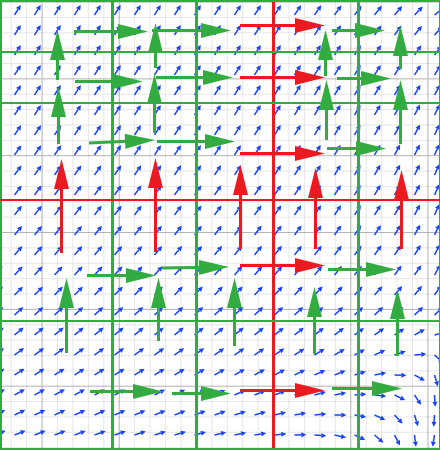
\includegraphics[scale=.40]{trans.png}
\end{center}
\vspace*{-0.5em}
\caption{Rectangular state space partitioning with $n = 4$. Green arrows are internal transitions, red arrows represent cross transitions.}
\label{fig:3dresults}
\end{figure}			
		
		
    \chapter{Algorithm}
    
    	In this chapter, we describe the distributed algorithm that computes the semantic function $\sem$. 
    	
    	\section{Distributed Environment}
    	
		In this section, we briefly describe the distributed environment assumed by our algorithm, in order to prevent any possible confusion.
		
		We assume a distributed environment with fixed number of reliable processes connected by reliable, order-preserving channels (The order preservation can be relaxed to some extent). We also assume that each process has a fixed identifier and the set of all process identifiers is equal to the result set of the partition function. Each process can communicate directly (using the function \method{Send}) with any other process (assuming it knows other process's identifier). We assume that each message can be transmitted in $O(1)$ time and all messages that can't be processed directly are stored in a buffer until they can be processed.		
		
		Several parts of the algorithm do not have explicit termination (they terminate by reaching deadlock - no messages are exchanged between processes). In such cases, suitable termination detection algorithm is employed to detect this deadlock and terminate computation properly. Our implementation uses Safra's algorithm \cite{safra} for this purpose, but the related code has been skipped for easier readability.
    	
		The algorithm is broken into two main parts. First describes the general outline of algorithm and is similar to basic CTL model checking. Second part describes how each of the supported temporal operators is processed. This part contains more detailed description of inter-process communication and operator specific data structures. To better reflect the distributed nature of the algorithm, description of each temporal operator routine is divided into three parts: Process variables, Initialization and Message handler. First section describes data structures stored in process memory available during whole computation. Initialization section is executed exactly once and no messages can be received until it's finished. Message handler defines what should happen when message is received.  
		
		\section{Algorithm Outline}
		
			In order to compute the assumption function $\as$ for the given Kripke structure, we compute the value of $\sem(\asemt)$ by exchanging relevant assumptions between processes. The main idea of the algorithm is described in Algorithm \ref{alg:general} and resembles other CTL model checking algorithms.
			
			\begin{algorithm}
			\label{alg:general}
			\begin{algorithmic}[1]
				\Procedure{CheckCTL}{$ \psi, \ks $}
					\State Partition $\ks$ into $\kf{1}{\ks}, \cdots, \kf{N}{\ks}$
					\ForAllPar  { $\kf{i}{\ks}$ where $i \in \{1, \cdots, N\} $}
						\State $ \as \gets \asemt$ 						
							\ForAll { $ i \leq | \psi | $ }					
									\ForAll { $ \varphi $ \textbf{in} $ cl(\psi) $ \textbf{where} $ | \varphi | = i $ }
									\Repeat
										\State $ \as \gets \sem(\as)  $
										\State exchange assumptions with other processes
									\Until{all processes reach fixpoint}
								\State set $\as(p, s, \varphi) = \false$ where $\as(p, s, \varphi) = \perp$
							\EndFor
						\EndFor						
					\EndForPar
					\State merge assumptions from all processes
				\EndProcedure			
			\end{algorithmic} 
			\end{algorithm}
			
			The algorithm starts by partitioning the Kripke structure into $N$ fragments. For each of these fragments, it initializes the assumption function to undefined values. After that, it traverses the structure of formula, starting from smallest formulas and uses previously computed results to process more complex formulas. 
			
			When function $\sem$ can't compute any new assumptions, fragments exchange relevant information. The loop terminates when no new information is being computed in any process even after information exchange. When this happens, we can guarantee that the formula holds only in states marked accordingly, so we remove all undefined values by marking them as false.						
			
		\section{Temporal Operators}
    
    		In this section, we describe how the $\sem$ is implemented for each of the temporal operators. In order to reduce communication overhead, we exchange relevant assumptions while also computing the function $\sem$. This way we can better spread in time the amount of required communication.
    		
    		Note that all of the following algorithms has implicit termination and therefore needs a proper termination detection algorithm to correctly terminate.
    		
    		We do not provide algorithm for boolean operators and atomic propositions, since these can be trivially deduced from the assumption function semantics.
    		
	   		\subsection{Exist Next Operator}
   			   			
   			   	\begin{algorithm}
   			   	\caption{Exists next}
				\begin{algorithmic}[1]
				\State $ \textbf{Process variables:} $
				\State $ \fullKf{i}{} $ \Comment{Kripke fragment}
				\State $ \phi = \ex{\varphi_1}  $ \Comment{CTL formula}
				\State $ \as $ \Comment{Initial assumption function}
				\State $ f $ \Comment {Partition function}
				\Procedure{Init}{}
					\ForAll {$(state, colSet)$ \textbf{in} $ initialStates(\varphi_1, \as) $}
						\ForAll { $ (pred, tranCol) $ \textbf{in} $ predecessors(state) $ }
							\State $ \Call{Send}{f(state), (pred, colSet \cap tranCol)} $
						\EndFor
					\EndFor
				\EndProcedure
				\Procedure{Receive}{$dest, colSet$}
					\State set $\as(p, dest, \varphi) = \true$ for all $p \in colSet$
				\EndProcedure
				\end{algorithmic}	
				\end{algorithm}
				
				%The simplest of temporal operators is the \ex{} operator. During initialization, all states and colours where $\phi$ holds are computed. For each of such states, all predecessors are considered and appropriate message that will cause assumption update is sent.
				
				If formula is marked as valid in state $s$ for colour $p$, it means a message containing such state and colour has been received. This can only happen if said state has a successor under colour $p$ where $\varphi_1$ holds. Therefore no false positive results are produced. Also, for each state where $\varphi_1$ holds for colour $p$, a message is sent for all predecessors of such state. Therefore all states where $\ex{\varphi_1}$ holds are labelled accordingly. Since all correct states are labelled and no false positives are possible, the algorithm is correct.
				
				In the worst case, algorithm has to send every colour over every transition, therefore worst case message complexity is $card(\trans{}_{i})$. In practice, message count is usually much lower, since multiple colours can be packed into one message.
				
				Assuming the validity of $\varphi_1$ is computed for all states, function $initialStates(\varphi_1, \as)$ can be computed in $O(|S_{i}| \cdot |\params|)$ time. The function $predecessors$ can be pre-computed for all states in $O(card(\trans{}_{i}))$ time. The procedure \method{Send} is called at most $card(\trans{}_{i})$ times and the parameter set intersection is at worst linear in the size of parameter space. 
				
				This would result in $O(|\params| \cdot card(\trans{}_{i}))$ time complexity. However, this can be further reduced to $O(card(\trans{}_{i}))$ since we can observe that for every predecessor where $|tranCol| > 1$, only one message is sent instead of $|tranCol|$ messages. The colour set intersection can also be performed in $O(|tranCol|)$ time. This means that the price of set intersection is amortized by the reduced number of transmitted messages. 
				
				
			
    		\subsection{Exist Until Operator}
    			
    			\begin{algorithm}
    			\caption{Exists until}
				\begin{algorithmic}[1]
				\State $ \textbf{Process variables:} $
				\State $ \fullKf{i}{} $ \Comment{Kripke fragment}
				\State $ \varphi = \eu{\varphi_1}{\varphi_2}  $ \Comment{CTL formula}
				\State $ \as $ \Comment{Initial assumption function}
				\State $ f $ \Comment {Partition function}
				\Procedure{Init}{}
					\ForAll {$(state, colSet) $ \textbf{in} $ initialStates(\varphi_2, \as) $}
						\State set $\as(p, state, \varphi) = \true$ for all $p \in colSet$
						\ForAll { $ (pred, tranCol) $ \textbf{in} $ predecessors(state) $ }
							\State $ \Call{Send}{f(state), (pred, colSet \cap tranCol)} $
						\EndFor
					\EndFor
				\EndProcedure
				\Procedure{Receive}{$s, colSet$}
					\State $ colSet \gets colSet \cap validColours(\varphi_1, s, \as)$
					\If{$ colSet \neq \emptyset $ \textbf{and} $ colSet \setminus validColours(\varphi, s, \as) \neq \emptyset $}
						\State set $\as(p, s, \varphi) = \true$ for all $p \in colSet$
						\ForAll {$(pred, tranCol) $ \textbf{in} $ predecessors(s) $ }
							\State $ \Call{Send}{f(pred), (pred, colSet \cap tranCol)} $
						\EndFor
					\EndIf
				\EndProcedure
				\end{algorithmic}
				\end{algorithm}	
			
				The \eu{}{} operator is a little more complex, but again fairly simple. The algorithm starts by computing all states and colours where $\varphi_2$ is true and marks them as valid. Starting from these states, a back-propagation of parameter sets along the reversed transitions is performed. During the computation, the propagated parameter set is updated to reflect the validity of $\varphi_1$ in examined state and the validity of transitions used along the path. Note that back-propagation is stopped as soon as there is no new information computed ($colSet$ is either empty or equal to already computed assumptions).
				
				Algorithm reaches deadlock, because each message either adds true values to the assumption function or does not trigger sending of new messages. Since we have a finite state and parameter space, we can't add true values to the assumption function forever, and therefore at some point, no new messages will be sent.
				
				Algorithm is correct, because $\varphi$ is marked as true in some state and parameter only if $\varphi_2$ holds there, or $\varphi_1$ is true in this state and a message is received from some of the state's successors indicating that $\varphi$ holds in said successor. Also, if $\varphi$ is marked as true in some state, all of it's predecessors are always notified about this update. 
				
				Worst case message complexity is $card(\trans{}_{i})$ because at worst, we have to send every colour along every transition.	Note that we do not use the same parametrised transition twice, because this would mean that $\varphi$ was also set true twice for the same state and colour (We prevent this using the condition on line 16).
				
				Because all general functions have linear or better complexity and we know that for each transition and parameter, only one message is sent, using similar argument as in analysis of $\ex{}$, we can show that the time complexity of this algorithm is $O(card(\trans{}_{i}))$. 
			
		    \subsection{All Until Operator}
		    
		    	\begin{algorithm}
		    	\caption{All until}
				\begin{algorithmic}[1]
				\State $ \textbf{Process variables:} $
				\State $ \fullKf{i}{} $ \Comment{Kripke fragment}
				\State $ \varphi = \au{\varphi_1}{\varphi_2}  $ \Comment{CTL formula}
				\State $ T = \trans{}_i $ \Comment{Uncovered edges}
				\State $ \as $ \Comment{Initial assumption function}
				\State $ f $ \Comment {Partition function}				
				\Procedure{Init}{}
					\ForAll {$(state, colSet) $ \textbf{in} $ initialStates(\phi_2, \as) $}
						\ForAll { $ (pred, tranCol) $ \textbf{in} $ predecessors(state) $ }
							\State $ \Call{Send}{f(state), (state, pred, colSet \cap tranCol)} $
						\EndFor
					\EndFor
				\EndProcedure
				\Procedure{Receive}{$d, s, colSet$}	
					\State $ T \gets T \setminus \{ (s, p, d) | p \in colSet \} $
					\State $ colSet \gets \{ p \in \params \mid p \in colSet \wedge \forall s' \in S : (s, p, s') \notin T \} $
					\State $ colSet \gets colSet \cap valid(\varphi_1, s, \as)$
					\If{$ colSet \neq \emptyset $ \textbf{and} $ colSet \setminus validColours(\varphi, s, \as) \neq \emptyset $}
						\State set $\as(p, s, \varphi) = \true$ for all $p \in colSet$
						\ForAll {$(pred, tranCol) $ \textbf{in} $ predecessors(s) $ }
							\State $ \Call{Send}{f(pred), (to, pred, colSet \cap tranCol)} $
						\EndFor
					\EndIf
				\EndProcedure
				\end{algorithmic}	
				\end{algorithm}
				
				The \au{}{} operator is the most complex one to handle. As opposed to \ex{}{}, which requires at least one valid successor to be true, \au{}{} requires that all successors of the specific node are valid. In order to compute such information, we create a copy of transition relation and call it $T$. 
				
				During the computation, $T$ is modified in such way, so that we can guarantee that if transition is not present in $T$, this transition does not exist or it leads to a state where either $\varphi_2$ or \au{\varphi_1}{\varphi_2} holds. This way, we are keeping track of all edges that can falsify the validity of $\varphi$ and therefore when a state has no successors in $T$, we can mark it as valid.

				Algorithm reaches deadlock thanks to the same argument as used in analysis of EU.
				
				Algorithm is correct, because a state and colour are marked as true only if they have no successors in $T$ and $\varphi_1$ is also true. A state and parametrisation has no successor in $T$ only if all transitions valid for said parametrisation lead to a state where either $\varphi_2$ or \au{\varphi_1}{\varphi_2} holds. If a state is marked as true for some parametrisation, or $\varphi_2$ is true in it, an appropriate message is sent to all of it's predecessors. This guarantees the removal of this transition from $T$. 
				
				Using the same argument as in analysis of the EU operator, we can show that the worst case message complexity of the algorithm is $card(\trans{}_{i})$. Worst case time complexity is $O(maxOutDegree(\trans{}_{i}) \cdot card(\trans{}_{i}))$. This is due to the fact that operation on line 16 needs to check all outcoming edges from state $s$ in order to confirm that they are removed from set $T$. This is not an optimal time complexity (other methods based on search for strongly connected components can solve this problem in linear time), however, implementing these methods in distributed environment would result in increased communication and synchronization overhead. Also, typical biochemical models have a guaranteed small average maximal out degree, so that it can be effectively considered a constant coefficient.
								
		\section{Merge Message Buffer}
			\label{sec:merge}

			The main argument of coloured model checking efficiency is based on the assumption that operations on parameter sets are in practice less expensive than graph traversal. However, even a simple model structure can easily break the computation into many simultaneous traversals. When two different colour sets are marked as valid in a state due to two distinct transitions, unfortunate timing can easily prevent these two colour sets from merging into one. This leads to two outgoing messages instead of one, which in the end results in two separate graph traversals instead of one. 
			
			In some cases, this simply cannot be avoided, since in order to know exactly when to wait for a merge and when to continue the traversal, we would basically have to solve the model checking problem. However, we can take advantage of the fact, that many messages cannot be processed directly at the time of arrival, since message processing can be a costly operation, especially when the transition system is being lazily calculated. Therefore we use a message buffer to store incoming messages that cannot be processed directly.
			
			These buffers can grow quite large during the computation and in extreme cases even outgrow the state space of the transition system itself. Of course, it would be easy to just slow down the creation of messages to prevent the buffers from growing. However, many messages in these buffers contain data that are either duplicate or can be merged into one message while maintaining correct semantics.
			
			In order to reduce the number of unnecessary graph traversals and reduce memory footprint of message buffers while maintaining good performance, we employ a merge message buffer as described in algorithm \ref{alg:buffer}. 
			
			In this text, we only provide the implementation for messages that contain destination node and colour set, as used in $\ex{}$ and $\eu{}{}$ operators. However, the implementation for messages used by $\au{}{}$ operator can be obtained trivially by replacing all occurrences of destination node with pair of destination and source nodes.
			
			\begin{algorithm}
			\label{alg:buffer}
			\begin{algorithmic}[1]
			\State $ \textbf{MergeBuffer} $
			\State $ Q \gets IterableHashMap $
			\Procedure{Insert}{node, colours}
				\If {$Q$ \textbf{hasKey} $node$}
					\State $current \gets Q.get(node)$
					\State $Q.replace(node, colours \cup current)$
				\Else
					\State $Q.insert(node, colours)$				
				\EndIf
			\EndProcedure
			\Procedure{Empty}{}
				\State \Return $Q.isEmpty()$
			\EndProcedure
			\Procedure{Take}{}
				\State $val \gets Q.interator().first()$
				\State $Q.remove(val.key)$
				\State \Return $val$
			\EndProcedure
			\end{algorithmic}				
			\end{algorithm}
			
			Observe, that the buffer is backed by an $IterableHashMap$. Compared to traditional $HashMap$, $IterableHashMap$ provides also an iterator on all of its key-value pairs. This gives us the ability to take one (non-deterministic) element out of the map in constant time. Considering a reasonable hash function on the node set, we can guarantee that each operation on the underlying $IterableHashSet$ can be done in constant time. Therefore the only interesting operation in terms of time complexity is the union of two colour sets, which can be done in $O(\params)$ time.
			
			It is important to note that the resulting buffer does not preserve the FIFO properties of a queue. However, this is not required by the algorithm (actually, performing a random search instead of classic DFS is considered a valid optimization heuristic).
			
			We do not provide exhaustive benchmark of our implementation, since the main priority of this work is the model checking algorithm itself. However, a comparison with linked queue and circular buffer on models tested in the Section \ref{sec:scale} showed, that merge queue easily outperforms both of them especially in highly distributed environments. Linked queue was usually two times slower while circular buffer managed to provide approximately 70-90\% of the merge buffer performance. 
			
			One reason for this, is the fact that more distributed computations have generally more cross transitions. This increases the cost of traversal compared to parameter set operations which in turn makes the merge buffer more effective. Also, the properties of this buffer allow in some cases for super-linear scalability, since greater number of processes can produce higher number of merged traversals. 			
	
	\chapter{Implementation}

		Our algorithm is implemented in a proof-of-concept distributed CTL model checker available in the GitHub repository of the Sybila organization\footnote{https://github.com/sybila/Distributed-CTL-Model-Checker/tree/cmsb2015}. In this chapter, we discuss the implementation details of this project. 
		
		Although the core model checking module is fully operational and stable, the project is still mainly in experimental phase, since new features, heuristics and modelling approaches are still being considered and re-evaluated.
		
		In order to provide greater flexibility and ease of development, majority of the project is implemented in Java. However, some parts still require C++ code reused from similar previous projects. The whole project is built using Gradle build system.
			
		The distributed environment is mainly by MPJ, Java implementation of standard MPI interface. However, the model checking algorithm itself does not depend on any concrete communication library and can be easily adapted to any similar distributed communication tool.
			
		The whole project is divided into several modules in order to maximize extensibility and modifiability during future de\-vel\-op\-ment. We will now discuss each of these modules.
			
		In order to provide user with easy way to input CTL formulas, project contains a CTL Parser module which implements a parser for modified formula specification language used in Biodivine \cite{biodivine}. 
				
		The original parser only supports LTL formulas, therefore the grammar has been modified to allow for CTL operators. However, user familiar with the original LTL syntax should have no problems adapting to the CTL syntax.
				
		The grammar is written in Antlr parser generator and apart from the whole range of CTL and boolean operators supports also boolean and float propositions.
				
		This module also handles the syntactic abbreviations as defined in section \ref{sec:ctl}.
				
			
		The algorithm described in this work is implemented in the core model checker module. It defines the interfaces and contracts representing the Kripke fragment, parameter set, partition function and inter-process communication.
				
			It is completely independent on the implementation of said interfaces, and therefore provides great flexibility and extensibility. This module also provides partial implementations of some of these interfaces to ease the development of new modules. 
				
			The termination detection algorithm designed by Safra \cite{safra} is also implemented here. The termination detection itself can't be easily overridden, however, the communication is again isolated into one, easily replaceable class, so the support for different communication libraries can be easily provided.
	
			ODE Abstraction module is based on the ODE state space generator from the LTL model checking tool Biodivine \cite{biodivine}. The code responsible for model parsing and abstraction calculation is reused directly and Java Native Interface (JNI) is used to extract resulting model into corresponding Java data structures.
				
			The state space generator responsible for evaluation of atomic propositions and computation of successors/predecessors is based on code from the Biodivine project. However, this section has been completely rewritten into Java and adapted to the CTL paradigm. This minimizes the number of slow JNI calls to existing C++ code. This new state space generator also features several bug fixes and speed optimizations.
				
			Module also implements the rectangular partition function as described in chapter \ref{chap:partitioning}. The parameter set is implemented using Google Guava Range Set, which provides great flexibility and huge feature set while maintaining good performance.
				
			Thomas Network module is based on the Thomas Network state space generator from the LTL model checking tool Parsybone \cite{parsybone}. Similarly to the ODE Abstraction module, most of the model parsing and preprocessing is done using the original code and extracted using JNI. 
				
			The parameter set is implemented using a EWAH Compressed Bitmap, which provides decent performance even on large parameter sets and is very easy to use. 
				
			At the moment of writing, this module does not provide any good partitioning implementation, since much of its functionality is still in development and most of the current implementation is subject to change. However, sequential computation on one processing node is fully supported.					
			
			Frontend module ties together the functionality of all modules into several runnable utilities. However, the documentation and general outline and output format of these tools have not yet been finalized and is subject to change. Therefore the code in this module should be taken more as an example of usage of different modules.	
				
	\chapter{Experimental Evaluation}

			The aim of this chapter is to demonstrate the applicability of our algorithm on two biologically relevant models. First model is fairly simple and is used for benchmarking purposes, since it can be easily scaled and modified while maintaining similar properties and structure. Second model exhibits non trivial behaviour and is used to demonstrate the ability of our method to correctly detect such behaviour. 
		
			\section{Scalability}	
				\label{sec:scale}
			
				We evaluate the scalability of the algorithm on an ODE model of reversible catalytic reaction with varying number of intermediate enzyme-substrate complexes.  Using this model, we can easily scale the number of intermediate products/variables ($N$), discretization thresholds ($T$) and unknown parameters. For simplicity, we assume that each variable is evaluated on the same amount of thresholds, which results in the total state space size of $(T - 1)^N$. 
				
				
				The benchmarks were performed on a cluster of 12 computational nodes, each equipped with 16 GB of RAM memory and a quad-core Intel Xeon 2Ghz processor. In order to focus on the distribution and not multi-core performance, we utilize only one core on each machine. However, note that the algorithm can be easily executed on a multi-core machine or a cluster of multi-core machines using each core as separate process. No other resource intensive software was running at these machines at the time of benchmarking.
				
				The model itself is described in the figure \ref{fig:model}. The first line represents a simplified chemical equation of the model. The following lines describe differential equations for every species. The last two lines describe used parameters. 				


				\begin{figure}
					\label{fig:model}
					\centering
					\underline{$S + E \rightleftharpoons ES_1 \rightleftharpoons \dots \rightleftharpoons ES_k \rightleftharpoons P + E$}\\
					$\dot{S}  =  0.1\cdot ES_1 - p_1\cdot E\cdot S$\\
					$\dot{E}  =  0.1\cdot ES_1 - p_2\cdot E\cdot S + 0.1\cdot ES_k - p_2\cdot E\cdot P$\\
					$\dot{ES_1} = 0.01\cdot E\cdot S - p_3\cdot ES_1 + 0.05\cdot ES_2$\\
					$\vdots $\\
					$\dot{ES_k} = 0.1\cdot ES_{k -1} - p_k\cdot ES_k + 0.01\cdot E\cdot P$\\
					\underline{$\dot{P}  =  0.1\cdot ES_k - p_{k+1}\cdot E\cdot P - 0.1\cdot P$}\\
					$p_1 = 0.01, p_2 = 0.01, p_3 = 0.2,$\\ $p_k = 0.15, p_{k+1} = 0.01$
					\caption{ODE model of reversible catalytic reaction}
				\end{figure}


				In the subsequent tables, we provide detailed information about the runtime of the distributed algorithm on various modifications of the model and a CTL formula $\ag{(P \leq 30)}$.  The value {\em N/A} represents a situation when the algorithm ran out of memory. The results have been obtained as an arithmetic mean of several experiments.
				
				They generally illustrate very good scalability in terms of evaluated model properties. Note that the number of parameters can change the structure of the transition system, which may result in shorter run times, as demonstrated in table \ref{tab:param}. Also note that in several occasions, especially when comparing single and dual machine experiments, the algorithm exhibits a super-linear speed-up. There are two main reasons of this behaviour. 
				
				First is the merge buffer as described in section \ref{sec:merge}, which can non-deterministically merge several traversals into one and therefore reduce expected overhead. Second is the garbage collector used by the Java Runtime Environment. Single machine experiments generally take up more memory, since the whole state space has to be stored on one computer. This leads to more aggressive garbage collecting and thus results in higher run times. On the other hand, when using high number of computational nodes, the garbage collection has only insignificant impact thanks to the high amount of available memory.
				
				\begin{table}
				\label{tab:param}
					\centering
					\setlength{\tabcolsep}{6pt}
					\begin{tabular}{|*{7}{c|}}
						%	\hline
						%	\multicolumn{7}{|c|}{times for model with 6 dimensions per 13 thresholds in seconds} \\
						\hline
							\# of params	& 1 	& 2 	& 3	& 4	& 5	& 6	\\
							%		(\# of states) & ($12^6$) & ($12^6$) & ($12^6$) & ($12^6$) & ($12^6$) & ($12^6$) \\
						\cline{1-1}
							\# of nodes	&	&	&	&	&	&	\\
						\hline
							1 & 6456	& {\em N/A} & {\em N/A} & {\em N/A} & {\em N/A} & {\em N/A} \\
							2	& 2610		& 6179			& 5089			& 	{\em N/A}				&	{\em N/A}					&	{\em N/A}					\\
							3	&	1696		&	4022			&	3661			&	3784			&	{\em N/A}					&	{\em N/A}					\\
							4	&	854			&	1759			&	2285			&	2454			&	{\em N/A}					&	{\em N/A}					\\
							5	&	683			&	1371			&	1365			&	1580			&	1736			&	{\em N/A}					\\
							6	&	499			&	1095			&	1019			&	1254			&	1609			&	1350			\\
							7	&	435			&	861				&	796				&	1023			&	1406			&	1340			\\
							8	&	292			&	642				&	650				&	853				&	1134			&	1118			\\
							9	&	258			&	439				&	630				&	752				&	983				&	962				\\
						 	10	&	232			&	418				&	557				& 637				&	839				&	822				\\
							11	&	198			&	347				&	516				&	553				&	784				&	679				\\
							12	&	177			&	329				&	420				&	562				&	759				&	660				\\
						\hline
					\end{tabular}\\[1em]
					\caption{The runtime in seconds for the model with 6 variables, 13 thresholds and different number of unknown parameters.}				
			\end{table}

			\begin{table}
				\centering
				\setlength{\tabcolsep}{6pt}
				\begin{tabular}{|*{5}{c|}}
					%	\hline
					%	\multicolumn{5}{|c|}{times for model with 1 unknown parameter in seconds} \\
					\hline
						\# of variables & 4 & 5 & 6 & 7 \\
						%(\# of states) & ($10^4$) & ($10^5$) & ($10^6$) & ($10^7$) \\
						\cline{1-1}
						\# of nodes & & & & \\
					\hline
						1	& 3.3 &	22 &	794 & {\em N/A}	\\
						2 &	3.3 &	12 &	489	& {\em N/A} \\
						3 &	3.5 &	9.5 &	253 & {\em N/A} \\	
						4 &	3.4 &	8.2 &	185 &	8571 \\
						5 &	2.7 &	8 &	112 &	6608 \\
						6 &	2.4 &	7.2 &	101 &	5291 \\
						7 &	2.7 &	7.3 &	77 &	3024 \\
						8 &	2.3 &	6.6 &	64 &	2630 \\
						9 &	2.3 &	6.3 &	55 &	2366 \\
						10 &	2.5 &	6.8 &	52 &	2081 \\
						11 & 2.7	&	6.2 &	47 &	1999 \\
						12 & 2.2	&	5.6 &	41 &	1828 \\
					\hline
				\end{tabular}\\[1em]
				\caption{The runtime in seconds for the model with 1 unknown parameter, 11 thresholds per the variable and different number of variables.}
			\end{table}
			
			\begin{table}
				\centering
				\setlength{\tabcolsep}{6pt}
				\begin{tabular}{|*{5}{c|}}
					\hline
						\# of thresholds & 10 & 11 & 12 & 13 \\
						%(\# of states) & ($9^6$) & ($10^6$) & ($11^6$) & ($12^6$) \\
						\cline{1-1}
						\# of nodes & & & & \\
					\hline
						1 &	274 &	794 &	1805 &	6456 \\
						2 &	196 &	489 &	1252 &	2610 \\
						3 &	84 &	253 &	570 &	1696 \\
						4 &	62 &	185 &	408 &	 854 \\
						5 &	51 &	112 &	280 & 683 \\
						6 &	40 &	101 &	226 &	499 \\
						7 &	33 &	77 &	192 &	435 \\
						8 &	29 &	64 &	161 &	292 \\
						9 &	26 &	55 &	145 &	258 \\
						10 &	24 &	52 &	108 &	232 \\
						11 &	23 &	47 &	94 &	198 \\
						12 & 22	 & 41	 & 96	&	177 \\
					\hline
				\end{tabular}\\[1em]
				\caption{The runtime in seconds for the model with 1 unknown parameter, 6 variables and different number of thresholds per variable.}
			\end{table}

			\newpage
						\newpage
									\newpage			\newpage
			\section{Case study}
				\label{sec:case}
			
				To demonstrate the applicability of the algorithm, we investigate a well-known ODE model \cite{bifurcation} which represents a two-gene regulatory network describing interaction of the tumour suppressor protein $pRB$ and the central transcription factor $E2F1$ (see Figure \ref{fig:genmodel} (left)). This network represents the crucial mechanism governing the transition from $G_1$ to $S$ phase in the mammalian cell cycle. In the $G_1$-phase the cell makes an important decision. In high concentration levels, $E2F1$ activates the $G_1/S$ transition mechanism. In low concentration of $E2F1$, committing to $S$-phase is refused and that way the cell avoids DNA replication.
				
				This mechanism is an example of \emph{bistable switch}. The system makes an irreversible decision to finally reach some of the two stable states. The model is represented by two differential equations as seen in Figure \ref{fig:genmodel}. In order to discretize this model, a piece-wise multi-affine approximation (PMA) has to be computed \cite{grosu}. In our experiments, we use 70 thresholds per each variable during this process. However, no significant change in results has been observed for higher threshold counts.
				
				On the resulting model, we can perform a coloured model checking of the formula $\varphi \equiv \ef{\ag{(\mathtt{high})}}\wedge \ef{\ag{(\mathtt{low})}}$ considering the initial parameter space ${\phi_{pRB}\in[0.001,0.025]}$. The atomic propositions  $\mathtt{low}$ and $\mathtt{high}$ characterise the location of expected regions of $E2F1$ stability. Based on the results reported in~\cite{bifurcation} we define the stable regions as $\mathtt{high}\equiv (E2F1>4 \wedge E2F1<7.5)$ and $\mathtt{low}\equiv ({E2F1>0.5} \wedge E2F1<2.5)$.
				
				As seen in figure \ref{fig:3dresults}, the computation has successfully discovered both stable areas and corresponding parameters, as well as area and parameters from which both stable states can be reached. However, note that due to over-approximation, only the stable areas are guaranteed to be true. 
				

\begin{figure}
  \begin{center}
       \vspace*{-6mm}
  \hspace*{-1cm}  \parbox{3.8cm}{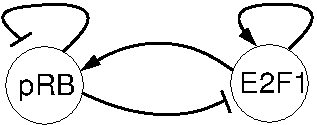
\includegraphics[scale=.7]{gs1net.pdf}}~
\parbox{6.5cm}{
\scriptsize
$$\begin{array}{c@{$\,=\,$}l}
\frac{d[pRB]}{dt} & k_1 \frac{[E2F1]}{K_{m1}+[E2F1]}\frac{J_{11}}{J_{11}+[pRB]}  - \phi_{pRB}[pRB]\\[1mm]
\frac{d[E2F1]}{dt} & k_p + k_2 \frac{a^2+[E2F1]^2}{K_{m2}^2+[E2F1]^2}\frac{J_{12}}{J_{12}+[pRB]} - \phi_{E2F1} [E2F1]
\end{array}$$
$a = 0.04$, $k_1=1$, $k_2=1.6$, $k_p=0.05$, $\phi_{E2F1}=0.1$ \\ $J_{11}=0.5$, $J_{12}=5$, $K_{m1}=0.5$, $K_{m2}=4$
}\\
    \end{center}
\caption{$G_1/S$ transition regulatory network and its ODE model taken from \cite{bifurcation}.}
\label{fig:genmodel}
\end{figure}


\begin{figure}
\begin{center}
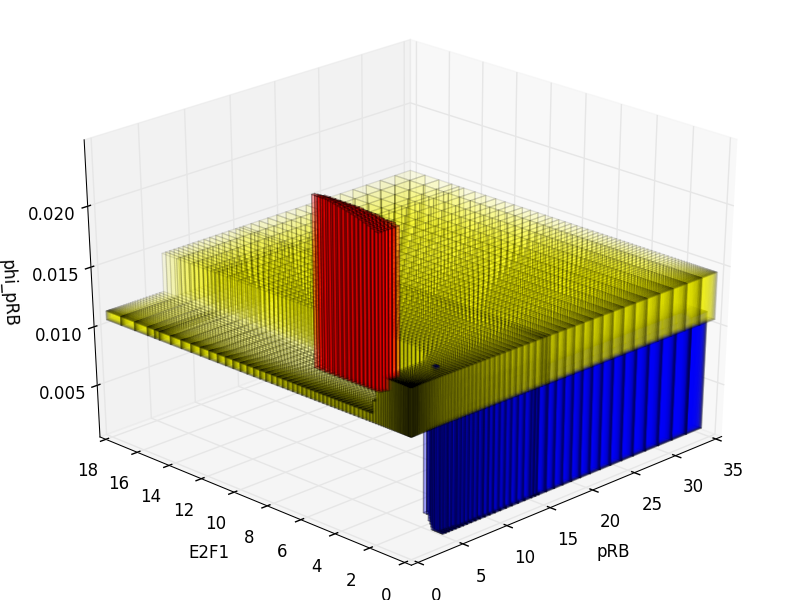
\includegraphics[scale=.35]{3d.png}
\end{center}
\vspace*{-0.5em}
\caption{Coloured model checking results. Red and blue parts
  correspond to the high and low stable regions, respectively. Yellow part
  displays the states where the overall \emph{bistable switch} formula $\varphi$
  holds.}
\label{fig:3dresults}
\end{figure}

	\chapter{Conclusion}
		
		The aim of this work was to design and implement a method that can efficiently solve parameter synthesis problem for biochemical models and CTL hypothesis. 
		
		We proposed an algorithm based on existing algorithms for distributed CTL model checking and coloured model checking of LTL formulas. The algorithm is given as pseudocode and we also provide a working implementation. The algorithm is not limited to the biochemical models and therefore has general applicability.

		We also proposed an efficient state space partitioning heuristic for ODE models and a merge buffer heuristic for reduction of unnecessary state space traversals.
				
		The provided implementation is oriented at biochemical models, provides support for two distinct modelling techniques, full range of CTL operators and features easily extensible modular architecture.
		
		We benchmarked the provided implementation and showed that the algorithm scales well with higher number of computation nodes and provides sufficient performance to investigate models with large state spaces, even though the exponential state space explosion still remains a problem. The applicability of the algorithm and applicability has been demonstrated on a biologically relevant model of bistable switch.
		
		In the future, the implementation can be optimized to provide even better performance and scalability, especially on multi-core architectures. Also support for different modelling techniques and partitioning heuristics can be implemented.
		
		Another possible direction of development would be a coloured symbolic model checking, which should provide even better performance compared to our explicit method, especially in terms of memory usage. 
			
					
    \bibliographystyle{ieeetr}  
	\bibliography{bibliography}	
	
    % Bibliography goes here
    % Index goes here (optional)
    \appendix
    \chapter{List of electronic attachments}
		\begin{itemize}
			\item Source code of the Implementation of the distributed memory coloured CTL model checker
		\end{itemize}
\end{document}
